%%%%%%%%%%%%%%%%%%%%%%%%%%%%%%%%%%%%%%%%%
% Arsclassica Article
% LaTeX Template
% Version 1.1 (10/6/14)
%
% This template has been downloaded from:
% http://www.LaTeXTemplates.com
%
% Original author:
% Lorenzo Pantieri (http://www.lorenzopantieri.net) with extensive modifications by:
% Vel (vel@latextemplates.com)
%
% License:
% CC BY-NC-SA 3.0 (http://creativecommons.org/licenses/by-nc-sa/3.0/)
%
%%%%%%%%%%%%%%%%%%%%%%%%%%%%%%%%%%%%%%%%%

%----------------------------------------------------------------------------------------
%	PACKAGES AND OTHER DOCUMENT CONFIGURATIONS
%----------------------------------------------------------------------------------------

\documentclass[
10pt, % Main document font size
a4paper, % Paper type, use 'letterpaper' for US Letter paper
oneside, % One page layout (no page indentation)
%twoside, % Two page layout (page indentation for binding and different headers)
headinclude,footinclude, % Extra spacing for the header and footer
BCOR5mm, % Binding correction
]{scrartcl}

%%%%%%%%%%%%%%%%%%%%%%%%%%%%%%%%%%%%%%%%%
% Arsclassica Article
% Structure Specification File
%
% This file has been downloaded from:
% http://www.LaTeXTemplates.com
%
% Original author:
% Lorenzo Pantieri (http://www.lorenzopantieri.net) with extensive modifications by:
% Vel (vel@latextemplates.com)
%
% License:
% CC BY-NC-SA 3.0 (http://creativecommons.org/licenses/by-nc-sa/3.0/)
%
%%%%%%%%%%%%%%%%%%%%%%%%%%%%%%%%%%%%%%%%%

%----------------------------------------------------------------------------------------
%	REQUIRED PACKAGES
%----------------------------------------------------------------------------------------

\usepackage[
nochapters, % Turn off chapters since this is an article        
beramono, % Use the Bera Mono font for monospaced text (\texttt)
eulermath,% Use the Euler font for mathematics
pdfspacing, % Makes use of pdftex’ letter spacing capabilities via the microtype package
dottedtoc % Dotted lines leading to the page numbers in the table of contents
]{classicthesis} % The layout is based on the Classic Thesis style

\usepackage{arsclassica} % Modifies the Classic Thesis package

\usepackage[T1]{fontenc} % Use 8-bit encoding that has 256 glyphs

\usepackage[utf8]{inputenc} % Required for including letters with accents

\usepackage{graphicx} % Required for including images
\graphicspath{{Figures/}} % Set the default folder for images

\usepackage{enumitem} % Required for manipulating the whitespace between and within lists

\usepackage{lipsum} % Used for inserting dummy 'Lorem ipsum' text into the template

\usepackage{subfig} % Required for creating figures with multiple parts (subfigures)

\usepackage{amsmath,amssymb,amsthm} % For including math equations, theorems, symbols, etc

\usepackage{varioref} % More descriptive referencing

\usepackage[numbers]{natbib}

\usepackage{xcolor}

%----------------------------------------------------------------------------------------
%	THEOREM STYLES
%---------------------------------------------------------------------------------------

\theoremstyle{definition} % Define theorem styles here based on the definition style (used for definitions and examples)
\newtheorem{definition}{Definition}

\theoremstyle{plain} % Define theorem styles here based on the plain style (used for theorems, lemmas, propositions)
\newtheorem{theorem}{Theorem}

\theoremstyle{remark} % Define theorem styles here based on the remark style (used for remarks and notes)

%----------------------------------------------------------------------------------------
%	HYPERLINKS
%---------------------------------------------------------------------------------------

\hypersetup{
%draft, % Uncomment to remove all links (useful for printing in black and white)
colorlinks=true, breaklinks=true, bookmarks=true,bookmarksnumbered,
urlcolor=webbrown, linkcolor=RoyalBlue, citecolor=webgreen, % Link colors
pdftitle={}, % PDF title
pdfauthor={\textcopyright}, % PDF Author
pdfsubject={}, % PDF Subject
pdfkeywords={}, % PDF Keywords
pdfcreator={pdfLaTeX}, % PDF Creator
pdfproducer={LaTeX with hyperref and ClassicThesis} % PDF producer
} % Include the structure.tex file which specified the document structure and layout

\hyphenation{Fortran hy-phen-ation} % Specify custom hyphenation points in words with dashes where you would like hyphenation to occur, or alternatively, don't put any dashes in a word to stop hyphenation altogether

%----------------------------------------------------------------------------------------
%	TITLE AND AUTHOR(S)
%----------------------------------------------------------------------------------------

\title{\normalfont\spacedallcaps{Restless: Why Do Elders Delay Retirement?}} % The article title

\author{\spacedlowsmallcaps{Alexey Filatov*}} % The article author(s) - author affiliations need to be specified in the AUTHOR AFFILIATIONS block

\date{} % An optional date to appear under the author(s)

%----------------------------------------------------------------------------------------

\begin{document}

%----------------------------------------------------------------------------------------
%	HEADERS
%----------------------------------------------------------------------------------------

\renewcommand{\sectionmark}[1]{\markright{\spacedlowsmallcaps{#1}}} % The header for all pages (oneside) or for even pages (twoside)
%\renewcommand{\subsectionmark}[1]{\markright{\thesubsection~#1}} % Uncomment when using the twoside option - this modifies the header on odd pages
\lehead{\mbox{\llap{\small\thepage\kern1em\color{halfgray} \vline}\color{halfgray}\hspace{0.5em}\rightmark\hfil}} % The header style

\pagestyle{scrheadings} % Enable the headers specified in this block

%----------------------------------------------------------------------------------------
%	TABLE OF CONTENTS & LISTS OF FIGURES AND TABLES
%----------------------------------------------------------------------------------------

\maketitle % Print the title/author/date block

%\setcounter{tocdepth}{2} % Set the depth of the table of contents to show sections and subsections only

%\tableofcontents % Print the table of contents

%\listoffigures % Print the list of figures

%\listoftables % Print the list of tables

%----------------------------------------------------------------------------------------
%	ABSTRACT
%----------------------------------------------------------------------------------------

\section*{Abstract} % This section will not appear in the table of contents due to the star (\section*)

Since the mid-eighties, both labor force participation and hours worked (for those who work) of seniors in US started to grow steadily after about a century of decline. There are various explanations put forward to account for this fact (such as increased life expectancy, moving from DB to DC pension plans, increased full retirement age), but the literature is lacking rigorous exploration of relative importance of these factors. This paper is intended to fill this gap.

%----------------------------------------------------------------------------------------
%	AUTHOR AFFILIATIONS
%----------------------------------------------------------------------------------------

{\let\thefootnote\relax\footnotetext{* \textit{Universitat Aut\'onoma de Barcelona, Barcelona, Spain}}}


%----------------------------------------------------------------------------------------

\newpage % Start the article content on the second page, remove this if you have a longer abstract that goes onto the second page

%----------------------------------------------------------------------------------------
%	INTRODUCTION
%----------------------------------------------------------------------------------------

\section{Introduction}
Around three decades ago labor force participation of persons aged 65 and older in the US hit the historical minimum at 11\%. Since then it was growing steadily and reached almost 20\% in 2014. On top of that, not only elderly participate in the labor force more, but they also work more as well, with average number of hours worked per week increased from 30 to 33 between 1984 and 2014. Previously observed pattern of abrupt retirement has also been changing, with more and more people approaching full retirement through a span of part-time job (\cite{Rupert2015}). With the large cohort of Baby Boomers currently entering this age, the elderly will comprise more and more significant part of the labor force, if the trends will continue. Several very important questions inevitably arise in this context. 

\textbf{Who exactly are those who delay retirement, by socio-economic status?} It is well-perceived that persons of different sexes, education level, marital status probably will behave differently on the labor market upon approaching the age of retirement. So what characterises those who delay retirement the best?

\textbf{What are the reasons that drive such a change in their behavior?} Numerous explanations of the trends have been put forward in the literature, but there is still lack of a rigorous analysis. What are the relative importance of the factors that affect the decision of an aged person to delay retirement?


\subsection{Employer pensions: Shift from defined benefit to defined contribution retirement plans (\cite{Clark2002}).} As opposed to defined benefit plan, defined contributions retirement plans stimulate participants to stay employed, as the benefits are based on amount contributed.
\subsection{Increased life expectancy.} Increase life expectancy means the necessity to finance more years of retirement. Coupled with the fact that health condition gets worse, and consequently medical expenditures grow rapidly at older age, this could lead to a desire to stay on the job longer. Despite the availability of Medicare at the age of 65, the amount of health expenditures not covered by Medicare is still substantial, even more so at older age, when health conditions become more severe.
\subsection{Social Security reforms. Increasing full retirement age and elimination of mandatory retirement (\cite{Clark2002}).} All of these act in a straightforward fashion. 
\subsection{Increasing medical expenditures.} Over the previous decades, the percentage of US GDP spent on health care has grown substantially. Although a part of individual medical expenditures is covered with insurance (if one has it), or Medicare after the age of 65, out-of-pocket spendings of individuals might still constitute  significant part of individual's spendings.
\subsection{High college premium.}
The high wage paid to college educated individuals might be one of the reasons that keep them from retirement. The data demonstrates that the large fraction of those who delay retirement have college education or higher.
\subsection{Decrease in the employer provided health care insurance.}



\textbf{How this change is affecting (and will likely continue to affect) the economy?} The range of potential effects and questions is large. How it affects inequality (including inequality in the narrow sense: among elderly), in terms of wage, earnings, wealth? Should government policies be aimed to promote employment among elderly (for example, through hiring subsidies)? 

\textbf{Moving against the general trend.} Even more surprising the increase in labo force participation of elderly looks in comparison to the fact that labor force participation of other age groups is actually decreasing at the time. The labor force participation of men was decreasing since the  middle of 20th century, whereas labor force participation of females slowed down or even reversed in early 2000's.

Existing literature on this topic is prevalently an empirical one. It currently lacks the quantitative model that can investigate the set of facts in unifying framework, as well as a possible structural model that can allow to compare the relative importance of the different factors affecting individual retirement decisions.
 
%----------------------------------------------------------------------------------------
%	Facts
%----------------------------------------------------------------------------------------

\section{Facts}

The data sample is extracted from March supplement of Current Population Survey and spans from 1964 to 2014. The population is split into four categories: 16 to 24 years old, 25 to 54 years old, 55 to 64 years old, and 65+ years. 

Four panels of Figure \vref{fig:oldonwork_all} are intended to give a broad idea of changes in each group's behavior.

\begin{figure}[h]
\centering 
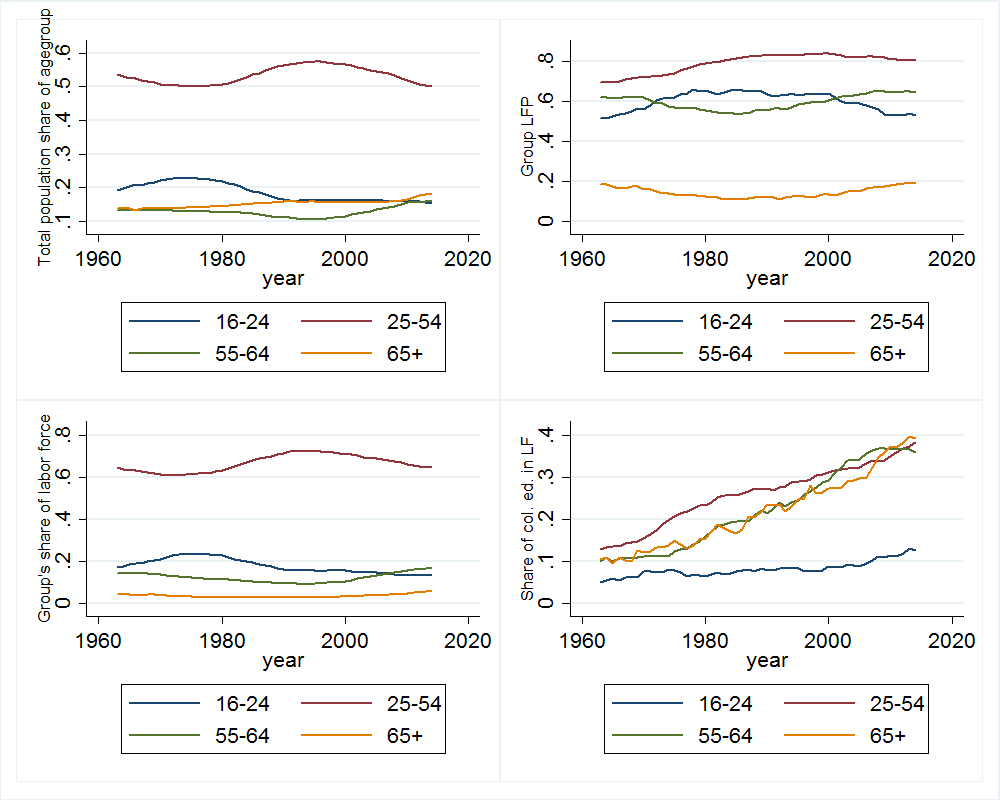
\includegraphics[width=1.0\columnwidth]{old_on_work.png} 
\caption{Labor force behavior of different age groups (CPS March supplement, 1963-2014, both sexes.)} % The text in the square bracket is the caption for the list of figures while the text in the curly brackets is the figure caption
\label{fig:oldonwork_all} 
\end{figure}
Top left panel shows that total population share of individuals aged 55+ has increased substantially in last two decades. Top right panel shows that labor force participation of individuals aged 55+ is increasing steadily since mid-eighties, which stands in contrast to labor force participation of other age groups. Bottom left panel shows that share of labor force that individuals aged 55+ constitute is again increasing since mid-eighties, whereas corresponding shares of other age groups are decreasing. Bottom-right panel represents the share of labor force that constitute individuals with at least college education. It is clearly seen that for each age group except for 16-24 years old the share of college educated persons increased dramatically since 1963 from about 12\% to almost 40\%.

\textbf{Counterfactual experiment.} In order to confirm that there is some behavioral change and not just composition effects, figure \vref{fig:counterfactual} presents a counterfactual experiment: keep the labor force participation as  in 1963, and change change the population shares of age groups. It clearly shows that there are behavioral changes. Although this figure doesn't give a clear picture of particular changes in LFP of elderly, it gives a broad picture of the dramatic changes that were overwhelming the US labor market since the sixties.
\begin{figure}[h]
\centering
\subfloat[Both sexes, 16+ years old.]{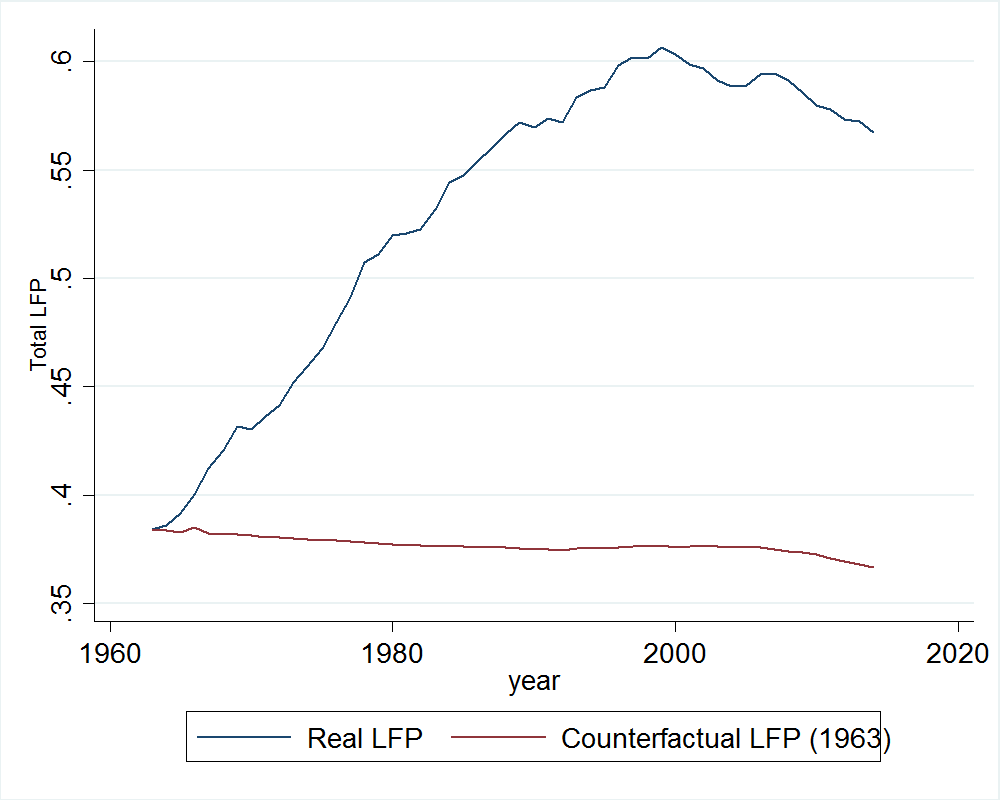
\includegraphics[width=.45\columnwidth]{counterfactual_lfp.png}} \quad
\subfloat[Only males, 16+ years old.]{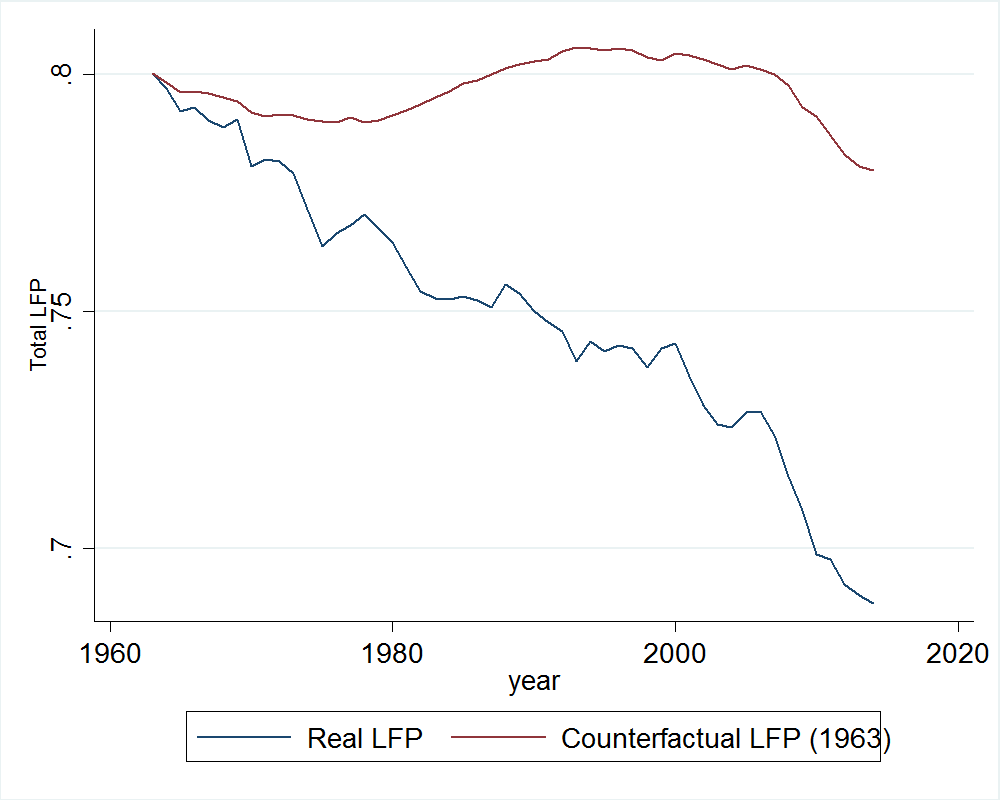
\includegraphics[width=.45\columnwidth]{counterfactual_lfp_male.png}} \\
\subfloat[Only females, 16+ years old.]{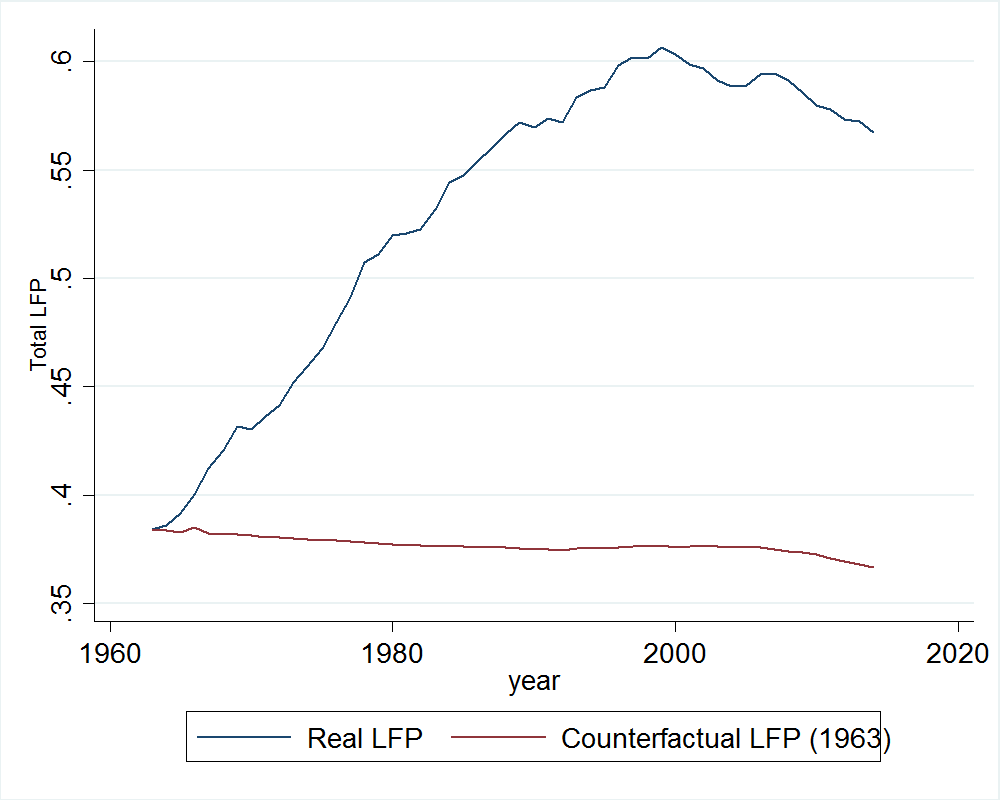
\includegraphics[width=.45\columnwidth]{counterfactual_lfp_female.png}} \quad
\caption[]{Counterfactual experiment.} % The text in the square bracket is the caption for the list of figures while the text in the curly brackets is the figure caption
\label{fig:counterfactual}
\end{figure}

\textbf{Older individuals work longer hours.} Figure \vref{fig:weeklyhours} represents change in labor supply in terms of weekly hours worked for college graduates and individuals without a college degree for the same time span. The increase in hours is visible for 55+ years old individuals and is more pronounced since the beginning of 2000s. This keeps for both educational categories.
\begin{figure}[h]
\centering 
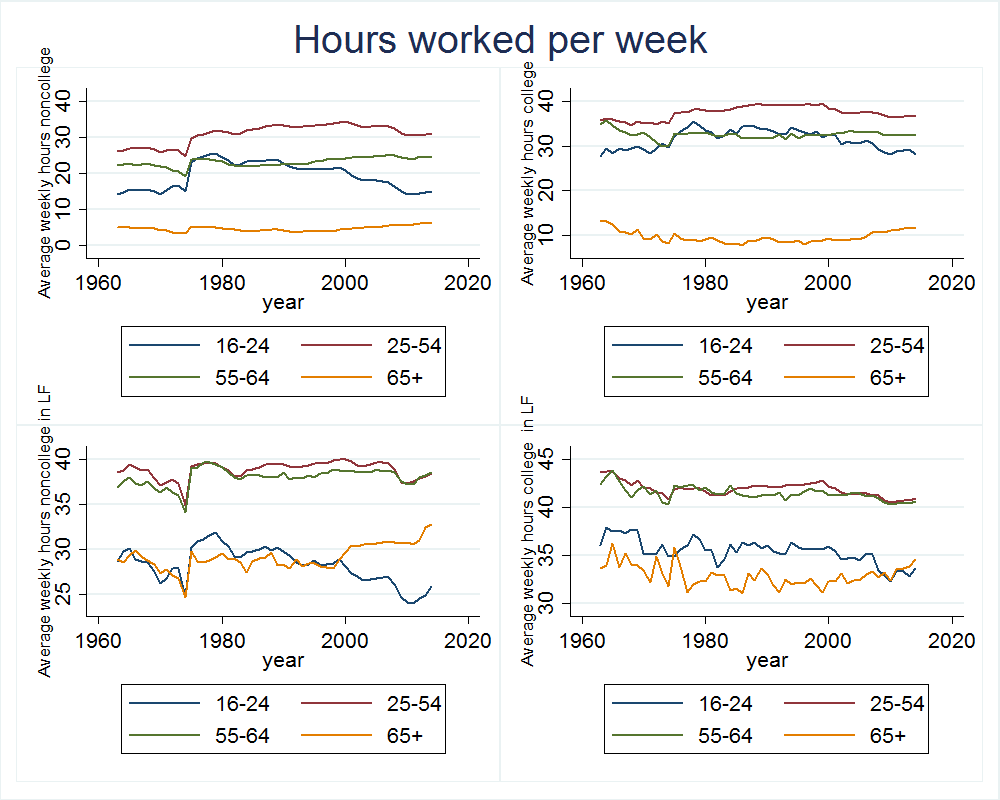
\includegraphics[width=1.0\columnwidth]{old_hours_supply.png} 
\caption{Weekly working hours.} % The text in the square bracket is the caption for the list of figures while the text in the curly brackets is the figure caption
\label{fig:weeklyhours} 
\end{figure}

\textbf{Older males and females behave similarly.} The well known and deeply investigated fact is that labor force participation of working age males is steadily decreasing since the middle of last century, whereas labor supply of females is has been increasing. The more surprising then comes the fact that for older individuals the patterns are quite the same: for both males and females aged 55+ their labor supply diminishes until roughly mid-eighties, and then comes up. This can be a mere coincidence, but also can be a sign of some deep process beyond this behavior, that differs from the processes that rule the labor supply of prime-age individuals.

\textbf{Education matters.} The increase in LFP of elderly is the more pronounced the higher is level of educational attainment of individual. The figures in the appendix demonstrate this fact. Furthermore, given that the individuals with at least college education constitute now more than 30\% of the total labor force, the clear conclusion is that more educated tend to stay in labor force longer. A number of things can lead to this fact. First, college educated got paid more, which gives them an incentive to stay longe in labor force. Second, they are more healthy. Third, the type of jobs college educated do are as a rule not physically demanding, hence they can perform it without significant decrease in productivity until older age. Fourth, the self selection into college assumes higher levels of productivity and self selection into later retirement. Fifth, the rise in assortative mating grants that the spouses of college educated individuals are often also college educated, and couples tend to coordinate retirement (however, Schirle (2008\cite{Schirle2008}) didn't find much of a result with her empirical specifications).

\textbf{Changes in retirement patterns.} Rupert and Zanell \cite{Rupert2015} introduce novel set of facts about the retirement behavior of youngest cohorts approaching the traditional retirement age. These facts stay in contrast to retirement patterns documented in previous literature. First, more and more individuals currently choose to retire gradually, passing through the period of part-time job. This contradicts the commonly accepted viewpoint of abrupt retirement. Second, the earnings of individuals aged 55+ go down, whereas hourly wage tend to grow for some time after the hours start to decline.  Burtless (2013) documents this fact as well.
%------------------------------------------------

\section{Literature Review}
There are number of papers that document the trend towards later retirement that started in 1980's.

Clark and Quinn (2002\cite{Clark2002}) is one of the first papers to document the trend reversal, with elimination of mandatory retirement,  social security amendments and changes in employer pensions being offered as possible reasons for it. Friedberg in 2007\cite{Friedberg2007} brief highlights the trend for males and females aged 55+. The paper identifies changes in public policy, private pensions and health care as a possible reasons for people to work longer. Juhn et al. (2006\cite{Juhn2006}) notes the reversal in the decline of labor force participation of older individuals and attributes it to the changes in social security as a possible explanation. DiCeccio et al. (2008\cite{DiCecio2008}) marks this trend as countervailing to the overall decline in the labor force participation during the previous decade, and along with the possible reasons mentioned above argues that increased life expectancy can play a role. 

Blau and Goodstein (2010\cite{Blau2010}) claim Social Security changes can account for 18-20\% of the change, but to the less extent  can explain the long decline in LFP of elderly throughout the 20th century. The counterfactual experiments they run suggest that under assumption that the marginal college attendee today may have lower ability than in previous periods when college attendance was less common, the chngin educational composition of the labor force can explain up to 100\% of the increase. 

Hurd and Rohwedder (2011\cite{Hurd2011}) use HRS data to study the effect of pensions (in particular, moving from DB to DC pension plans) on labor force participation of elderly. The main finding is that changes in the prevalence of DB and DC pensions are associated with changes in retirement rates. The authors' simulations demonstrate that shift from DB to DC between 1992 and 2004 will increase labor force participation rates of people in their 60s by about 2.5 percentage points.

Schirle (2008\cite{Schirle2008}) identifies a coordination in retirement schedule among spouses as another important reason and finds that husband's response to wives' labor force participation can explain 25\% of the increase.

Maestas and Zissimopoulos (2010\cite{Maestas2010}) summarize recent literature on the topic, dividing possible causes to supply (skill and educational composition of the workforce, spousal complementarity in retirement decision, changes in social security, mortality decline) and demand (skill-biased technological change, shift form defined benefit plans to defined contribution plans, reduction in employer-provided health insurance) sides.

Burtless (2013\cite{Burtless2013}) finds that those who stay in the labor force longer tend to be more productive than those who leave, thus finding little evidence the aging workforce has hurt aggregate productivity.

\section{Model}
This is a partial equilibrium life-cycle model. Individuals are heterogenous in several aspects: they differ by educational attainment (at this point college/non-college), which is exogenous and given at "birth"; the agents are of different sexes. The hetrogeneity affects their survival hazard and wage schedule. Earnings, health and medical expenditures of an agent are subject to idiosyncratic uncertainty; the details of these processes are described further in text.

\subsection{Demography}
An individual live for maximum of $J = 75$ periods, which means that at age $100$ person dies with certainty.

Agents start their lives at the age of 25, which corresponds to $t = 1$. The initial distribution of wages for the agents of different genders and educational levels is exogenously given and to be calibrated to the data.

 There is a survival hazard rate  $s_t = s(t,e,g,h_t)$ every period that depends on individuals age $t<J$, education, gender and current health status $h$ (see DeNardi et al (2010)\cite{DeNardi2010}). 

\subsection{Health status}
I model the health of individual following DeNardi et al. (2010) \cite{DeNardi2010}. Every period of life agent face two possible health statuses: healthy ($h=1$) and unhealthy ($h=0$), which affects agent's contemporaneous utility. Health is one of the sources of idiosyncratic uncertainty in the model, with current status being dependent on previous health, gender, age and education, with transition probabilities given by:
\begin{equation*}
\pi_{j,k}^{t,e,g} = Pr(h_{t+1} = k|h_t= j, t,e,g), \ j,k\in\{0,1\}
\end{equation*}

\subsection{Utility}
Each period an agent has to make a choice over allocation of time unit it owns between leisure and labor. In order to model the retirement, there is a lower bound $\bar{l}\ge0$ to the possible amount of working time supplied (this number is going to be calibrated to the data), below which an individual is considered out of labor force. Retirement is a form of non-participation (see French (2005) \cite{French2005}). Note that agents can re-enter labor force. 

 Individuals enjoy contemporaneous utility from consumption, leisure and health $u(c,l,h)$. Upon death, an individual derives utility from leaving a bequest described by function $B(a,\tau)$ of assets at the time of death and taxes.
\begin{equation}
\max_{c_t,l_t,h_t}E_{P,H,M}\sum_{t=1}^J\beta^{t-1}\prod_{k=0}^{t-1}s_{k,e,g}\left(s_{t,e,g}u(c_t,l_t,h_t)+(1-s_{t,e,g})B(a_t,\tau)\right)
\end{equation}
The expectation is taken with respect to agent's productivity, health status, and medical expenditure shock. Future is discounted by common discount factor $\beta$. 

Bequest function $B(a)$ takes form that is common in the literature (see Fench (2005) \cite{French2005}, De Nardi (2010) \cite{DeNardi2010}):
\begin{equation}
B(a) = \eta\frac{(a+d)^{1-\sigma}}{1-\sigma},
\end{equation}
where $\eta$ is the magnitude of the bequest motivation, and $d$ is curvature of bequest function.

The particular functional form of contemporaneous utility function  is a combination of (Kitao (2015)\cite{Kitao2015} and DeNardi et al. (2010)\cite{DeNardi2010}):
\begin{eqnarray*}
u(c,l,h) = \delta(h)\frac{[c^{\gamma}(1-l-I(l>\bar{l})\cdot \kappa_{e,g})^{1-\gamma}]^{1-\sigma}}{1-\sigma},
\end{eqnarray*}
where $I(l>\bar{l})$ is an indicator that takes value of $1$ if an individual participates in the labor market, and $0$ oterwise, and $\kappa_{e,g}$ is the cost of participation in the labor market, that depends on gender and education level. \textcolor{red}{Note that $\kappa$ does not depend on age for purposes of identification.} The dependence of utility on health status  $\delta(h)$ is modelled following DeNardi et al. (2010)\cite{DeNardi2010} and Palumbo (1999)\cite{Palumbo1999}:
\begin{equation*}
\delta(h) = 1+\delta h,
\end{equation*}
so that when health is good ($h=1$) agent gains boost to utility.


\subsection{Wages}
Agents get paid according to exogenously given wage profile which depends on agent's education, gender and age. Corresponding wage profiles will be taken from the data. To be precise, for each combination of education (college/noncollege), gender (male/female) and age (25 to a max of 100).

\subsection{Earnings and productivity}
The agent earns $y_t^{t,e,g} = z_t l_t w^{t,e,g}\times I(l>\hat{l})$, where $w^{t,e,g}$ ia a point of a corresponding wage profile, $z$ is idiosyncratic productivity and $I(l>\hat{l})$ is indicator that person works more than minimal hours. This productivity consists of persistent and transitory components: 
\begin{eqnarray*}
z_t = \omega_t + \varepsilon_t, \ \varepsilon_t\sim \mathcal{N}(0,\sigma_{\varepsilon})  \\
\omega_t = \omega_{t-1} +\nu_t, \ \nu_t\sim\mathcal{N}(0,\sigma_{\nu})
\end{eqnarray*}
The errors $\varepsilon_t$ and $\nu_t$ are uncorrelated and iid across individuals (the differences between groups by age/gender/education are captured by different wage profiles).

 \textcolor{red}{\textbf{Problem:} how to estimate productivity process from MEPS data. Possibly, need to use PSID for this.}

\subsection{Medical expenditures}
Agent's out-of-pocket expenses (part of the total expenses not covered by Medicare, Medicaid or personal insurance, plus insurance premium paid by the agent) $m_t$ depend on health status, age, gender and education in the following way (see DeNardi et al. (2010) \cite{DeNardi2010}):
\begin{equation*}
\ln m_t = m(t,e,g,h) + \sigma(t,e,g,h)\times \psi_t 
\end{equation*}
Idiosyncratic component $\psi_t$ is assumed to be decomposed as in French and Jones (2004) \cite{French2004}.
\begin{eqnarray*}
\psi_t = \zeta_t + \xi_t, \   	\xi_t \sim N(0,\sigma_\xi^2) \\
\zeta_t = \rho_m\zeta_{t-1} + \epsilon_t, \   \epsilon_t \sim N(0,\sigma_\epsilon^2)
\end{eqnarray*}
 \textcolor{red}{\textbf{Problem:} MEPS data is a collection of short 2-year-long panels. Is it enough for identification?}

\subsection{Agent's budget constraint}

\begin{eqnarray*}
c_t + a_{t+1} +m_t = a_t+Y(ra_t+y_t+b_t,\tau)  \\
a_{t+1}\ge0
\end{eqnarray*}

Here, $y_t$ is labor income, $a_t$ is agent's assets at period $t$, $r$ is risk-free rate of return, $b_t$ is composite of different kinds of benefits, social security and pensions (described in details below) and $\tau$ is a tax schedule (to be described more carefully).  $Y$ is a function mapping sum of agent's labor income, asset return, government transfers (including social security) and pensions into a disposable income given current tax schedule.

\subsection{Benefits}
Benefits $b_t$ is a complex object. It includes a government-provided ``consumption floor'' (see \cite{DeNardi2010}), Social Security payments for eligible individuals, Medicare services after the age of 65, employer-provided pensions, third-party medical insurance.
\begin{equation*}
b_t = b_t^{Ma} + b_t^{ss}\times S_t+b_t^{pb}
\end{equation*}
\subsubsection{Consumption floor}
A way to think of the ``consumption floor'' $b_t^{Ma}$ is as of Medicaid insurance for low-income agents. It is necessary to make it consistent with public transfer programs.
\begin{eqnarray*}
b_t^{Ma} = \max\{0,\underline{c}+m_t - [a_t(1+r(1-\tau_a)) +y_t]\} \\
c_t = \underline{c} \ \text{if} \ b_t^{Ma} > 0  \\
a_{t+1} = 0 \ \text{if} \ b_t^{Ma} > 0  
\end{eqnarray*}

\subsubsection{Social Security}
At the age 62 ($t\ge37$) an individual can apply for retirement social security benefits, that are going to be paid to her/him through the rest of his/her life. Benefit application $S_t\in\{0,1\}$ is yet another decision individual makes on top of consumption, leisure and amount of assets.
It will depend on \emph{individual history} of earnings througout the carreer before retirment (Average Indexed Monthly Earnings, to be exact; see French (2005) \cite{French2005}). In fact, a person can work and receive Social Security benefits simultaneously. However, for beneficiaries of Social Security earnings test taxes labor income and benefits at very high level. Description of earnings test mechanism and discussion of its importance will follow.
\subsubsection{Pension Benefits}
Pension benefits are different from social security in that they are provided by empoyer. Like Social Security, pensions are illiquid until certain age (depending on particular pension plan) and depend on individuals earning history (typically, on years of service at the particular firm). I can borrow the ideas on how to construct pension from French (2005) \cite{French2005}.

\subsection{Modelling behavioral changes: exogenous data}
So far, the model described above is static in the sense that many primitivs of the model supposed to be taken from the data (e.g. survival hazards, wage profiles, benefit rules). However, in order to model behavioral changes, I need to add certain dynamics to it. In order to do that, there going to be several cohorts in the model, which are indexed by $n<N_g$. For every particular cohort, I'm going to construct the following exogenous profiles from the data. 
\begin{itemize}
\item \emph{Medical expenditures.} The cost of medicial services was growing rapidly in US in the last few decades. Despite the increase in Medicare and Medicaid coverage, it is highly probable that out-of-pocket expenditures constitue larger ang larger parts of medical expenses of consequent generations.
\item \emph{Survival hazard.} Take a person born, say, in $1920$. It is clear that survival hazard for the person is quite different than the one for the person born in 1950, but not that much different for the persons born in $1915$ or $1925$. So what I will try to do is to construct a few cohorts, with a mean birth years separated by 15-20 years, and construct survival profiles for them. I should take into account gender differences and the fact that more educated persons on average earn more, ang in general more healthy, as well as advances in medical science and changes in consciousness about healthy lifestyle.
\item \emph{Wage profiles.} Again, wage profile for a person born in $1920$ is quite different that for the person born in $1950$ (e.g. rise in returns to education, job polarization etc.). So I will try to construct those too.
\item \emph{Benefits.} Each of three parts of $b_t$ changed over the years. For example, Medicare coverage grow over the years.
\item \emph{Earnings test.} In year $2000$, the earnings test was eliminated for those who work after normal retirement age. This may present a strong incentive to work after normal retirement age. 
\end{itemize}

Upon constructing these profiles, I can solve the model and simulate labor supply choices of individuals under different regimes, as well as conduct counterfactual experiments.

\subsection{Dynamic programming problem}
The problem of indvidual in recursive formulation is presented below. Here I suppress the indices, which only characterize exogenously given structures:
\begin{itemize}
\item year of model calibration;
\item gender index;
\item education index.
\end{itemize}
These characteristics are static in the sense that they only affect agents givens, such as mean wage profile, government benefits, survival hazards. Given these objects, agent's state consists of its current age $t$, current level of assets $a$, idiosyncratic productivity $z$, health status $h$, medical expenditure $m$, level of accumulated labor income $\bar{y}$. Given the current state, agent chooses level of consumption, labor supply and assets to save:

\begin{equation}
V(t,a,z,h,m,\bar{y},S) = \max_{c,l,a',S'}\{u(c,l,h) + \beta s_t  E_{P,H,M} V(t+1,a',z',h',m',\bar{y}')\}
\end{equation}
subject to 
\begin{eqnarray*}
c + a' +m = a+Y(ra+y+b+\upsilon,\tau)
a'\ge0 \\
y = z w l \times I(l>\hat{l}) \\
\bar{y}' = f(\bar{y},y)\\
b = b^{Ma}+b^{Mc} + b^{ss}\times S\times I(t>37)+b^{pb}+b^{i} \\
S' = \max\{S',S\}
\end{eqnarray*}
Here, $f(\bar{y},y)$ is a function that describes $AIME_t$ (Average Indexed Monthly Earnings), which is average over $35$ highest earning years. For $0\le t \le 35$, function just calculates average earnings. For $t>35$ it checks if current level of income is higher than the lowest level of annual income in one of the previous years, and recalculates $AIME$ accordingly.  

\section{Calibration and Estimation}
This section outlines assumptions in the current paper and describes approach to calibration and estimation of the model.
The main assumptions are:
\begin{enumerate}
\item Preferences parameters of the agents in the model are similar for the different cohorts. This means in terms of preferences agents who are aged $55+$ in, say, 1985, are similar to those aged $55+$ in 2005.
\item The source of change in agent's behavior are changes in exogenous processes: survival hazard, medical expenditures, earnings, benefits provision, social security policies, tax regime.
\end{enumerate}

\subsection{General approach}
The problem at hand is to model the labor supply behavior of $55+$ year old individuals on intensive (hours worked per week) and extensive (participation decision) margins under different conditions with regard to differences in multiple processes mentioned above (survival hazard, medical expenditures etc). I am approaching the problem in several steps.
\begin{enumerate}
\item Fully calibrate model to fit the labor force participation behavior of individuals in year 1996 (the first year available at MEPS-HC dataset). In particular, this includes the estimation of individual preference parameters, that will be used in further calculatons. This is going to be done by Method of Simulated Moments (as it customary in the literature). The details of the procedure will be described further.
\item Once preference parameters are calibrated, for each year of observation available in the data I will recalibrate all exogenous processes in the model (survival hazards, medical expenditures etc.). Upon finishng the calibration, I will simulate a large number of households for each available data year, and compare the behavior of model households to the real ones. I will be able to see which part of the change in labor force participation decisions can be explained by these exogenous factors.
\item I can also conduct counterfactual experiments, shutting down certain channels of influence and comparing the results. For example, in year $2000$ I can recalibrate all exogenous processes except survivl hazard, keeping that one similar to $1996$, thus observing the relative importance of changes in expected longevity on labor supply decisions. 
\end{enumerate}

\subsection{Details of Estimation Procedure}
I will follow he procedure of DeNardi (2010) et al \cite{DeNardi2010}, French (2005) \cite{French2005} and use a two-step method of simulated moments. But first, I list the parameters I need to estimate and exogenous profiles that I'm going to feed to a model to be able to solve it.


\subsection{Data}
The data I plan to use for the estimation of the model is Household Component of Medical Expenditures Panal Survey (MEPS-HC) data. MEPS bagan in 1996 and is a nationally representative survey of the U.S. civilian noninstitutionalized population. The design of survey is two-year-long overlapping panel: every year, a panel of households is selected, and data for them is collected for two years. The survey has a very detailed individual level information, including data on income, education, health, and very thorough information about health insurance and expenditures. The informaion on medical expenditures is a primary reason for choosing this particular data set. 

%------------------------------------------------

\section{Appendix A. Notation.}

\begin{center}
	\begin{tabular}{| l | l |}
	\hline
	Variable & Meaning \\
	\hline
	$t$ & Age \\
	$J$ & Maximum age \\
	$s_{t,e,g}$ & Survival hazard \\
	$a_{t}$ & Asset level \\
	$e$ & Education level \\
	$g$ & Gender \\
	$h_{t}$ & Health status \\
	$\pi$ & Health transition probability \\
	$\bar{l}$ & Lower bound on hours worked \\
	$B$ & Bequest function \\
	$\eta$ & Magnitude of bequest motivation \\
	$d$ & Curvature of bequest function \\
	$\delta(h)$ & Health modulator of utility \\
	$\kappa$ &  Fixed cost of work \\
	$z_{t}$ & Idiosyncratic productivity \\
	$w_{t,e,g}$ & Wage profile \\
	$\omega$ & Persistent component of idiosyncratic productivity \\
	$\varepsilon_t$ & Transitory component of idiosyncratic productivity \\
	$\nu_t$ & Error term in AR1 productivity process \\
	$m_t$ & Out-of-pocket medical expenditures \\
	$\sigma$ & Intensity of AR1 process of medical expenditures \\
	$\tau_x$ & Various tax rates \\
	$b_x$ & Various benefits \\
	$\underline{c}$ & Consumption floor \\
	$\theta(t,h)$ & Medicare coverage \\
	$S$ &  Benefit application choice \\
	\hline
	\end{tabular}
\end{center}



%----------------------------------------------------------------------------------------
%	BIBLIOGRAPHY
%----------------------------------------------------------------------------------------

\renewcommand{\refname}{\spacedlowsmallcaps{References}} % For modifying the bibliography heading

\bibliographystyle{apa}

\bibliography{old_on_work} % The file containing the bibliography

%----------------------------------------------------------------------------------------

\end{document}